\chapter{Results}
\label{c:result}

\section{Datasets}

%
% GSE52194 Breast cancer
% GSE52778 Airway Muscle and Asthma
%

Two RNA-Seq datasets and one DNA-Seq datasets from Gene Expression Omnibus
(GEO) were used for the demonstration of BioCloud. GSE52194
\cite{eswaran2012:transcriptomic} was a transcriptome profiling dataset of
human breast cancer. mRNA profiles of 17 breast tumor samples of three
different subtypes (TNBC, non-TNBC and HER2-positive) and normal human breast
organoids (epithelium) samples (NBS) were sequenced using Illumina HiSeq 2000
sequencer. Full sample list can be found in Table~\ref{tab:dataset-breast}.
Raw sequence reads were obtained from NCBI Sequence Read Archive (SRA), thus
their FASTQ file names were based on their SRA accession ID. In GSE52194 breast
cancer dataset, condition was defined to be the cancer subtype of the sample.

\begin{table}[!htbp]
    \caption[Experiment design of breast cancer GSE52194]{
        Experiment design of breast cancer dataset GSE52194.
    }
    \label{tab:dataset-breast}
    \centering
    \begin{threeparttable}
        \begin{tabular}{llr}
            \toprule
            Condition & Sample name & SRA ID and filename \\
            \midrule
            NBS      & NBS1      & SRR1027188 \\
            NBS      & NBS2      & SRR1027189 \\
            NBS      & NBS3      & SRR1027190 \\
            TNBC     & TNBC1     & SRR1027171 \\
            TNBC     & TNBC2     & SRR1027172 \\
            TNBC     & TNBC3     & SRR1027173 \\
            TNBC     & TNBC4     & SRR1027174 \\
            TNBC     & TNBC5     & SRR1027175 \\
            TNBC     & TNBC6     & SRR1027176 \\
            Non-TNBC & Non-TNBC1 & SRR1027177 \\
            Non-TNBC & Non-TNBC2 & SRR1027178 \\
            Non-TNBC & Non-TNBC3 & SRR1027179 \\
            Non-TNBC & Non-TNBC4 & SRR1027180 \\
            Non-TNBC & Non-TNBC5 & SRR1027181 \\
            Non-TNBC & Non-TNBC6 & SRR1027182 \\
            HER2     & HER2-1    & SRR1027183 \\
            HER2     & HER2-2    & SRR1027184 \\
            HER2     & HER2-3    & SRR1027185 \\
            HER2     & HER2-4    & SRR1027186 \\
            HER2     & HER2-5    & SRR1027187 \\
            \bottomrule
        \end{tabular}
    \end{threeparttable}
\end{table}


Another RNA-Seq dataset, GSE52778 \cite{himes2014:rnaseq}, is a transcriptome
profiling dataset of human airway smooth muscle (HASM). mRNA profiles of 4 male
white donors' HASM cells treated with four treatment conditions were sequenced
using Illumina HiSeq 2000 sequencer with Illumina TruSeq assay, four treatment
conditions being: no treatment (Untreated); treatment with Albuterol (Alb);
treatment with Dexamethasone (Dex); treatment with simultaneous Albuterol and
Dexamethasone (Alb\_Dex). Full sample list can be found in
Table~\ref{tab:dataset-airway}. Raw sequence reads were obtained from SRA thus
sample raw FASTQ files are renamed using their SRA accession ID.

\begin{table}[!htbp]
    \caption[Experiment design of GSE52778 airway muscle dataset]{
        Experiment design of GSE52778 airway muscle dataset.
    }
    \label{tab:dataset-airway}
    \centering
    \begin{threeparttable}
        \begin{tabular}{llr}
            \toprule
            Condition & Sample name & SRA Accession ID \\
            \midrule
            Untreated & N61311\_Untreated  & SRR1039508 \\
            Untreated & N052611\_Untreated & SRR1039512 \\
            Untreated & N080611\_Untreated & SRR1039516 \\
            Untreated & N061011\_Untreated & SRR1039520 \\

            Dex       & N61311\_Dex        & SRR1039509 \\
            Dex       & N052611\_Dex       & SRR1039513 \\
            Dex       & N080611\_Dex       & SRR1039517 \\
            Dex       & N061011\_Dex       & SRR1039521 \\

            Alb       & N61311\_Alb        & SRR1039510 \\
            Alb       & N052611\_Alb       & SRR1039514 \\
            Alb       & N080611\_Alb       & SRR1039518 \\
            Alb       & N061011\_Alb       & SRR1039522 \\

            Alb\_Dex  & N61311\_Alb\_Dex   & SRR1039511 \\
            Alb\_Dex  & N052611\_Alb\_Dex\tnote{$\dagger$} & SRR1039515\tnote{$\dagger$} \\
            Alb\_Dex  & N080611\_Alb\_Dex  & SRR1039519 \\
            Alb\_Dex  & N061011\_Alb\_Dex  & SRR1039523 \\
            \bottomrule
        \end{tabular}
        \begin{tablenotes}
        \item[$\dagger$] This sample was excluded from the later-on analyses
            since its pair-end sequencing reads were mismatched.
        \end{tablenotes}
    \end{threeparttable}
\end{table}


% TODO: how deep is the sequencing depth of these WES samples?

The DNA-Seq dataset used in the demonstration was a human whole exome
sequencing done in our lab. Exome sequencing of 5 members from the same family
using Illumina HiSeq 2000 sequencer. The study aimed to find the common
variants shared in this family.



\section{Account registration and user dashboard}

A new user account was registered on BioCloud using email
\texttt{demo@biocloud.liang2.io}. Screenshots of the registration process are
shown in Figure~\ref{fig:biocloud-signup}, which resemble the process on common
websites. Most of the user inputs were sanity checked and validated, as shown
in Figure~\ref{fig:biocloud-signup}(b). After user completed the form, a
verification email was sent to the registered email address so as to make sure
all future email notifications can reach the user. A fixed message is displayed
on all pages of BioCloud if the user does not complete the email verification,
as shown in Figure~\ref{fig:biocloud-signup}(c).
Figure~\ref{fig:biocloud-signup}(d) shows the content of the verification
email, where an uniquely HMAC-based verification link was given. After clicking
on the link, user completed the verification and the fixed message for
verification was gone, as shown in Figure~\ref{fig:biocloud-signup}(e).

\begin{figure}[!p]
\centering
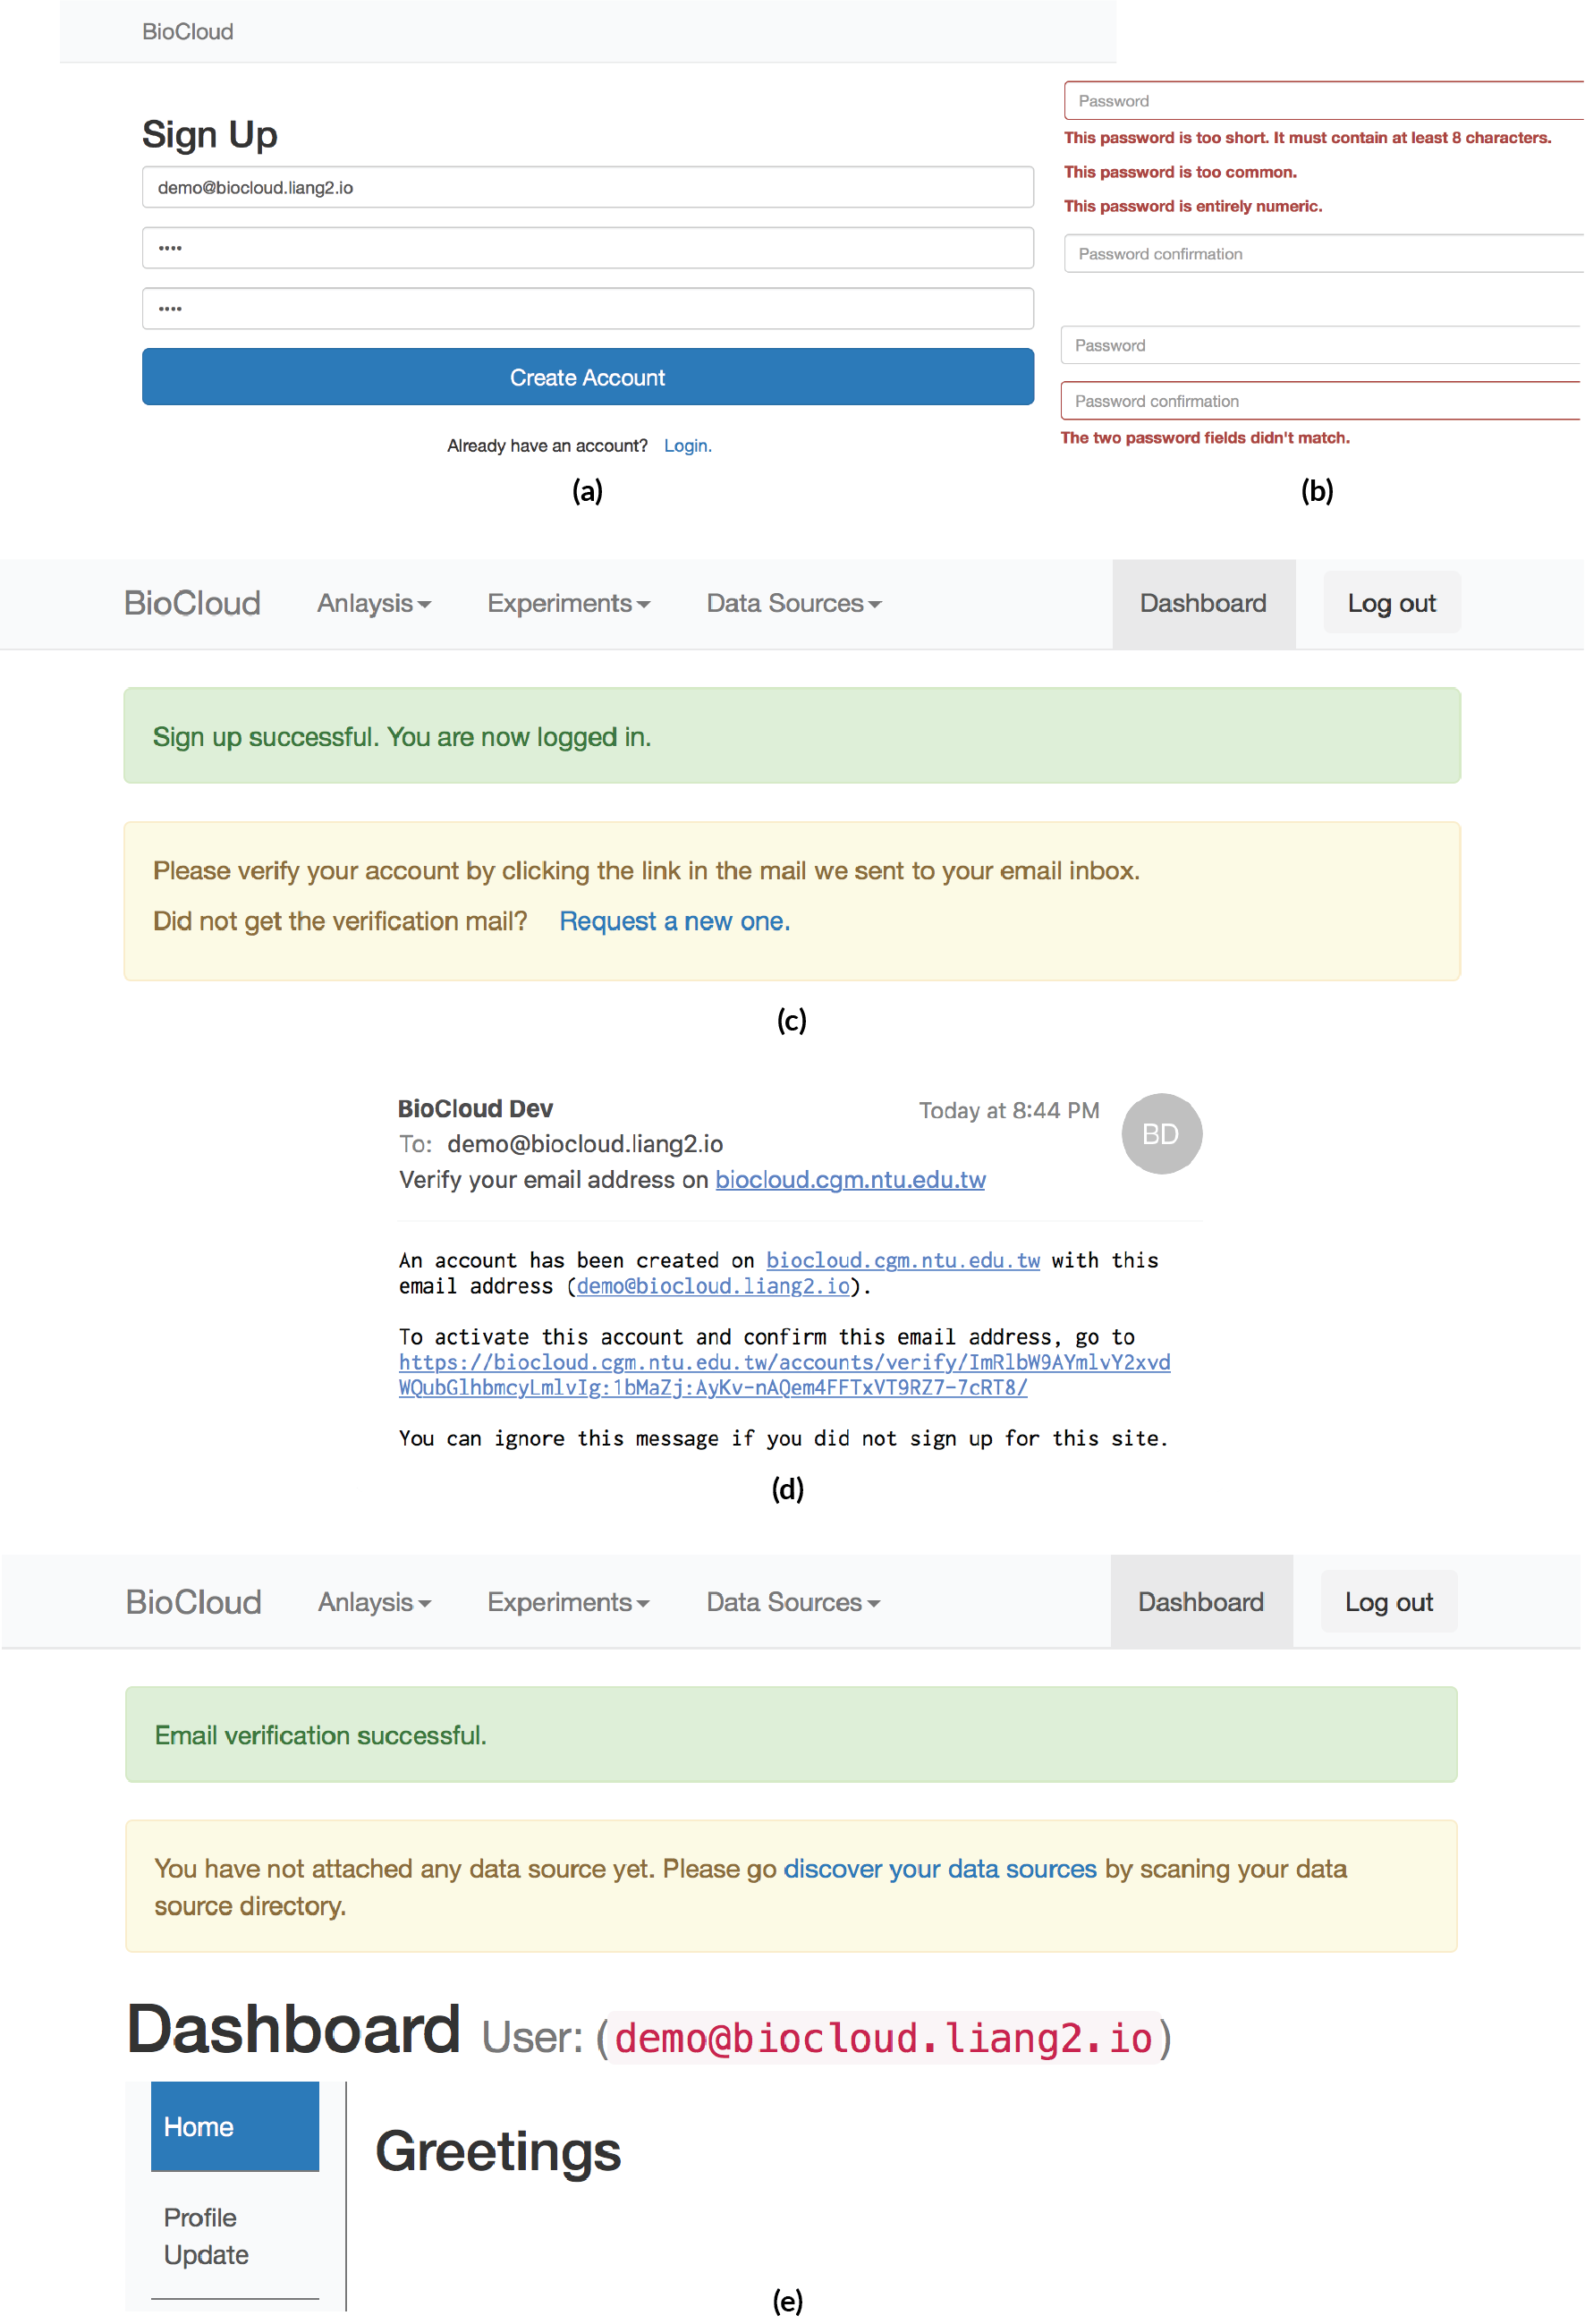
\includegraphics[width=1\textwidth]{images/biocloud_signup}
\caption[Account registration on BioCloud]{
    Account registration on BioCloud.
    (a) Registration form.
    (b) Password validation check.
    (c) Welcome screen after signup with action hint messages.
    (d) Verification email.
    (e) Welcome screen after email verifiction.
}
\label{fig:biocloud-signup}
\end{figure}


A user dashboard is available for user-related settings as shown in
Figure~\ref{fig:biocloud-dashboard}(b). User profile including user name and
authentication number (more on Section~\ref{s:report-result-access}) can be
updated here. Password can be changed via the link in the password section in
profile update, as shown in Figure~\ref{fig:biocloud-dashboard}(b). For staff
and superuser with special permission, they can access to the admin interface
of BioCloud in user dashboard via an extra tab ``Admin'', as shown in
Figure~\ref{fig:biocloud-dashboard}(d). Admin interface will be introduced in
Section~\ref{s:biocloud-admin}.

\begin{figure}[!p]
\centering
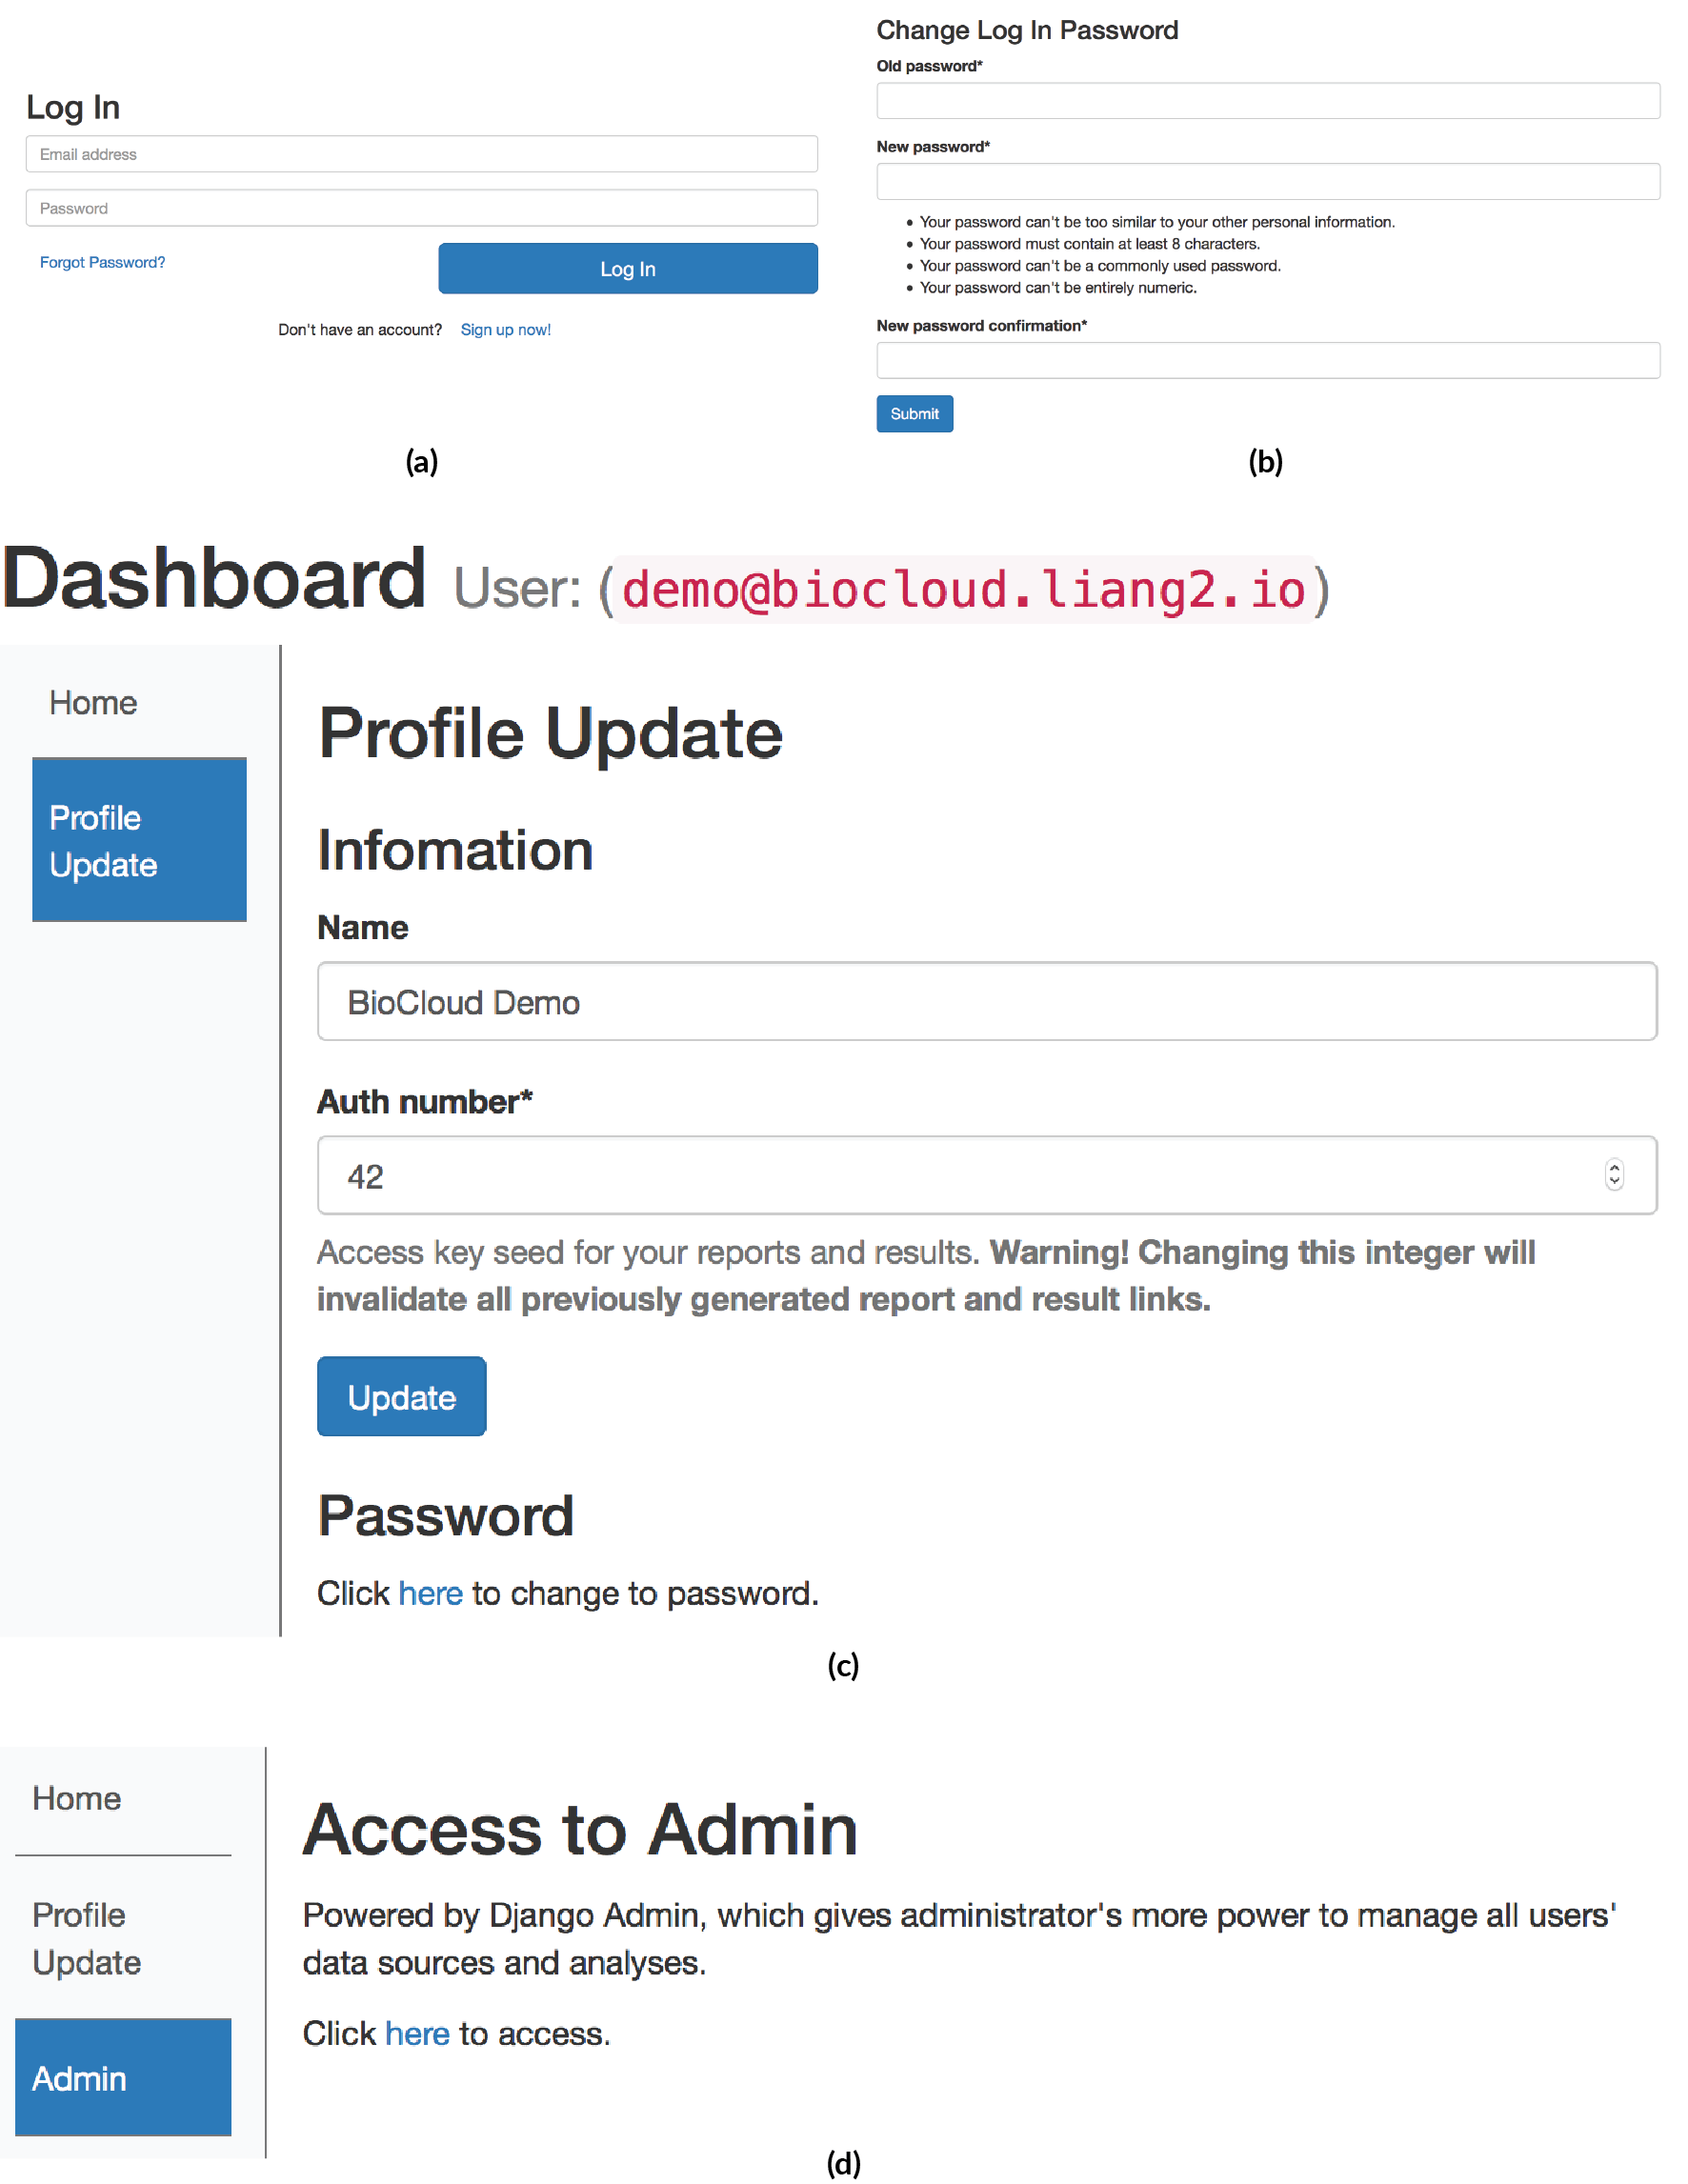
\includegraphics[width=1\textwidth]{images/biocloud_dashboard}
\caption[Login and user dashboard on BioCloud]{
    Login and user dashboard on BioCloud.
    (a) Login form.
    (b) Password change form available through profile update.
    (c) Profile update form.
    (d) For staff and superuser's dashboard, an extra tab to the admin
    interface is shown.
}
\label{fig:biocloud-dashboard}
\end{figure}





\section{Data source discovery}

As a newly registered user, a message was always shown to hint user to attach
their data sources to BioCloud. User can find their specific data source folder
from menu Data Source \textrightarrow List, as shown in
Figure~\ref{fig:biocloud-data-source}(b). For the demo user, location of the
data source folder on BioCloud server was:

\begin{CVerbatim}[fontsize=\small]
/biocloud/data_sources/2/
\end{CVerbatim}

\vspace{-1em}\noindent
After new data sources were added, BioCloud updated its database by comparing
the data sources in record with that in current folder.  All new discovered
data sources will be listed with guess of sample name and file type, as shown
in Figure~\ref{fig:biocloud-data-source}(a). User can pass the SHA2-256
checksum value for each file computed locally. BioCloud computed the checksum
of these files and compared the value with that supplied by the user. User can
check and update the detail of their recorded data sources, as shown in
Figure~\ref{fig:biocloud-data-source}(b). BioCloud also guessed the strand for
pair-end FASTA/Q files. The information was recorded at the metadata column in
JSON format.

\begin{figure}[!tbp]
\centering
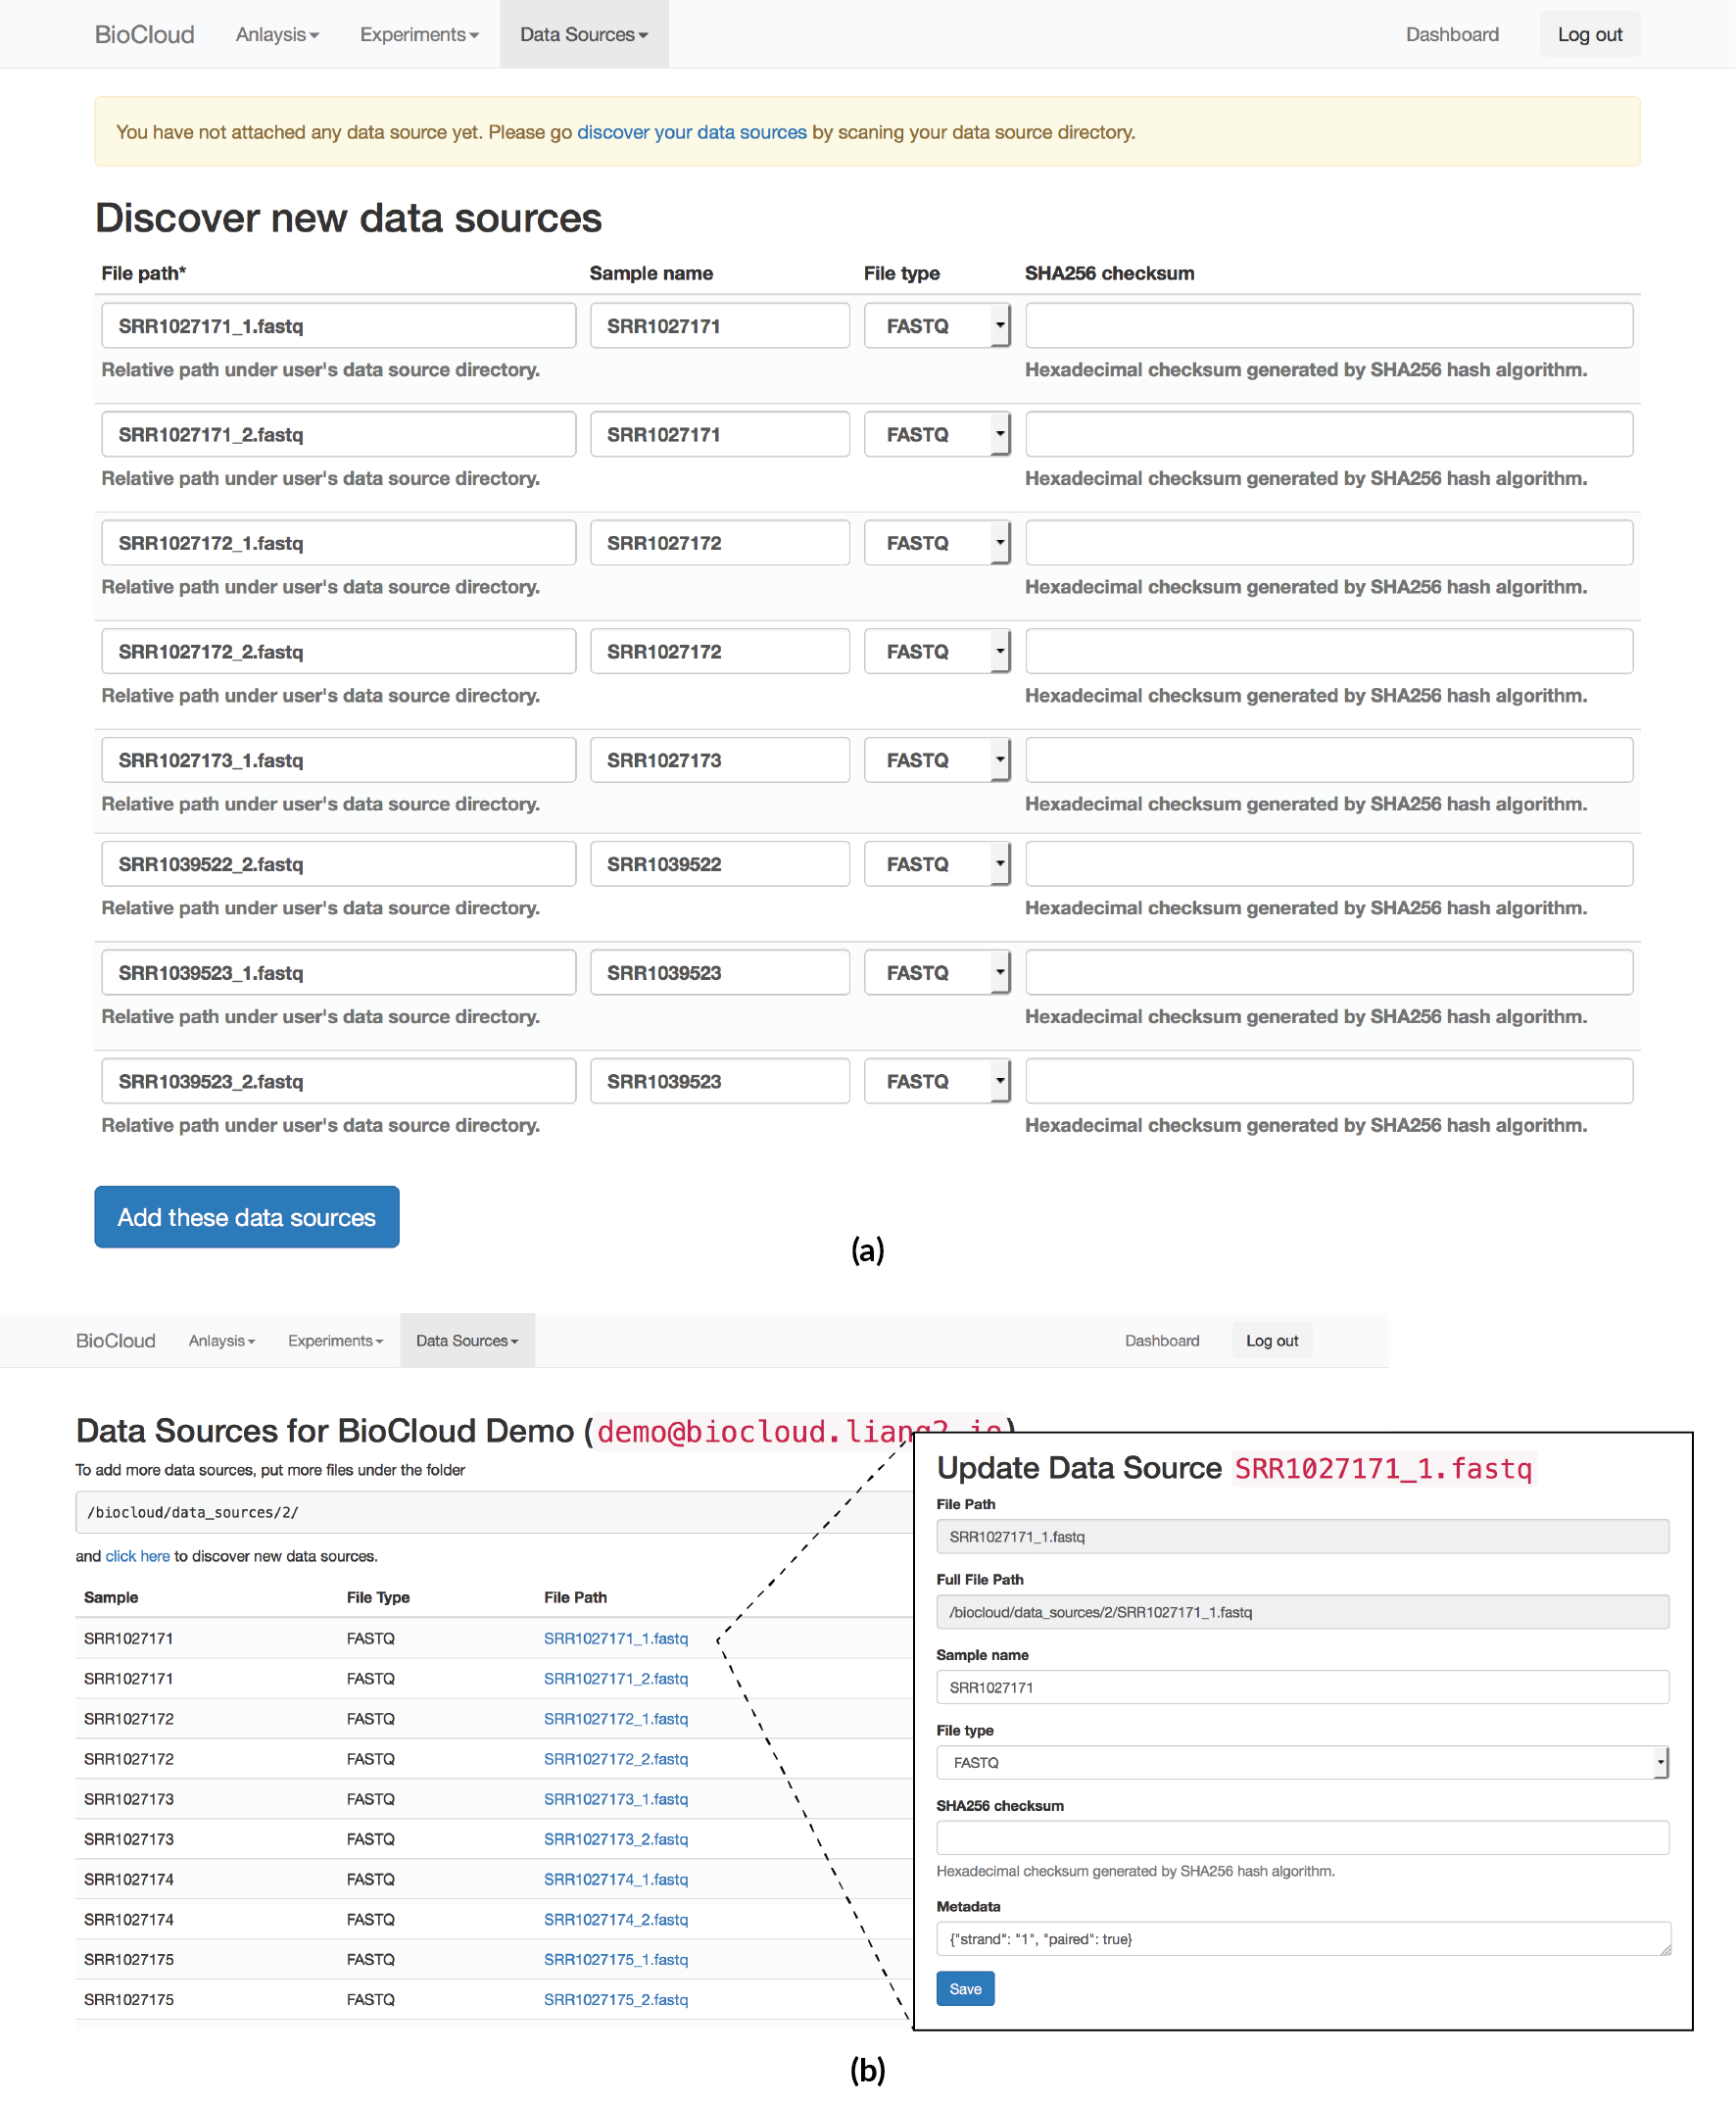
\includegraphics[width=1\textwidth]{images/biocloud_data_source}
\caption[Data source management on BioCloud]{
    Data source management on BioCloud.
    (a) Discovery of new ata sources.
    (b) List and detail view of data sources.
}
\label{fig:biocloud-data-source}
\end{figure}





\section{Experiment design}

Figure~\ref{fig:biocloud-experiment-design}.

% condition
\begin{figure}[!tbp]
\centering
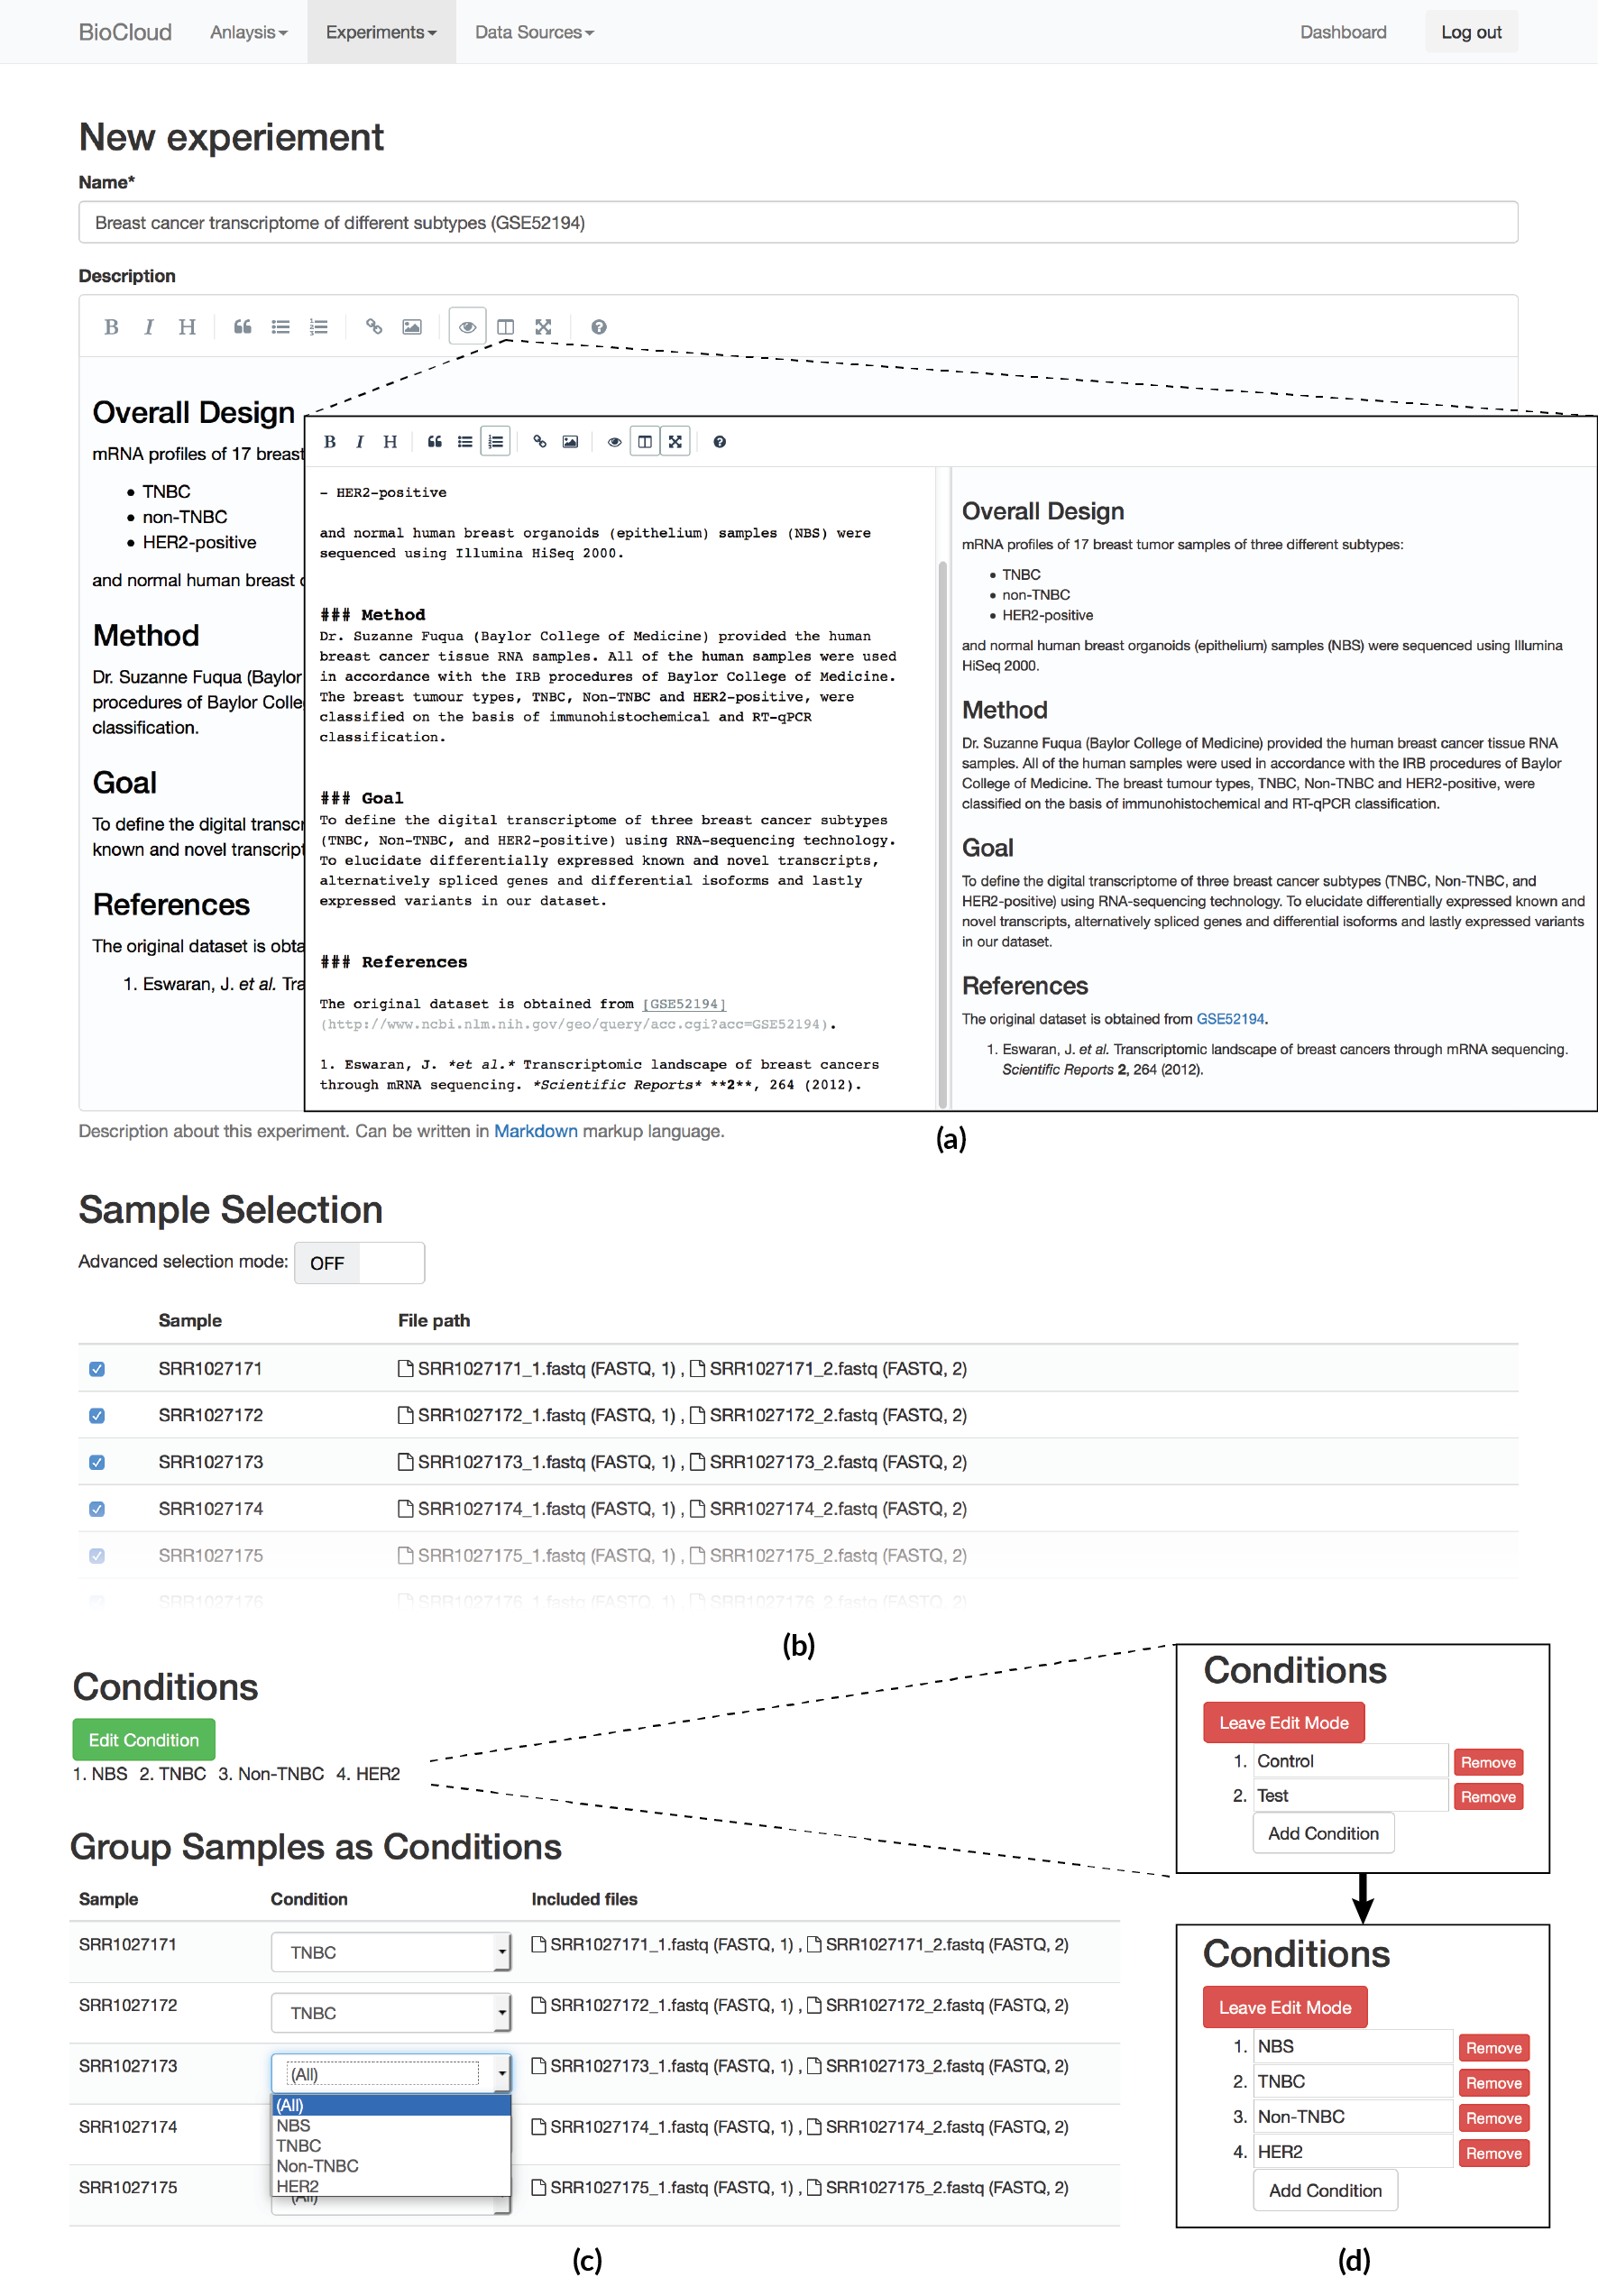
\includegraphics[width=1\textwidth]{images/biocloud_experiment_design}
\caption[Experiment design on BioCloud]{
    Experiment design on BioCloud.
    (a) Description Markdown editor in full screen.
    (b) Upper half of the experiment design form.
    (c) Condition assignment of samples.
    (d) Condition design.
}
\label{fig:biocloud-experiment-design}
\end{figure}


% simple and advanced mode
Figure~\ref{fig:biocloud-experiment-sample-condition}.

\begin{figure}[!tbp]
\centering
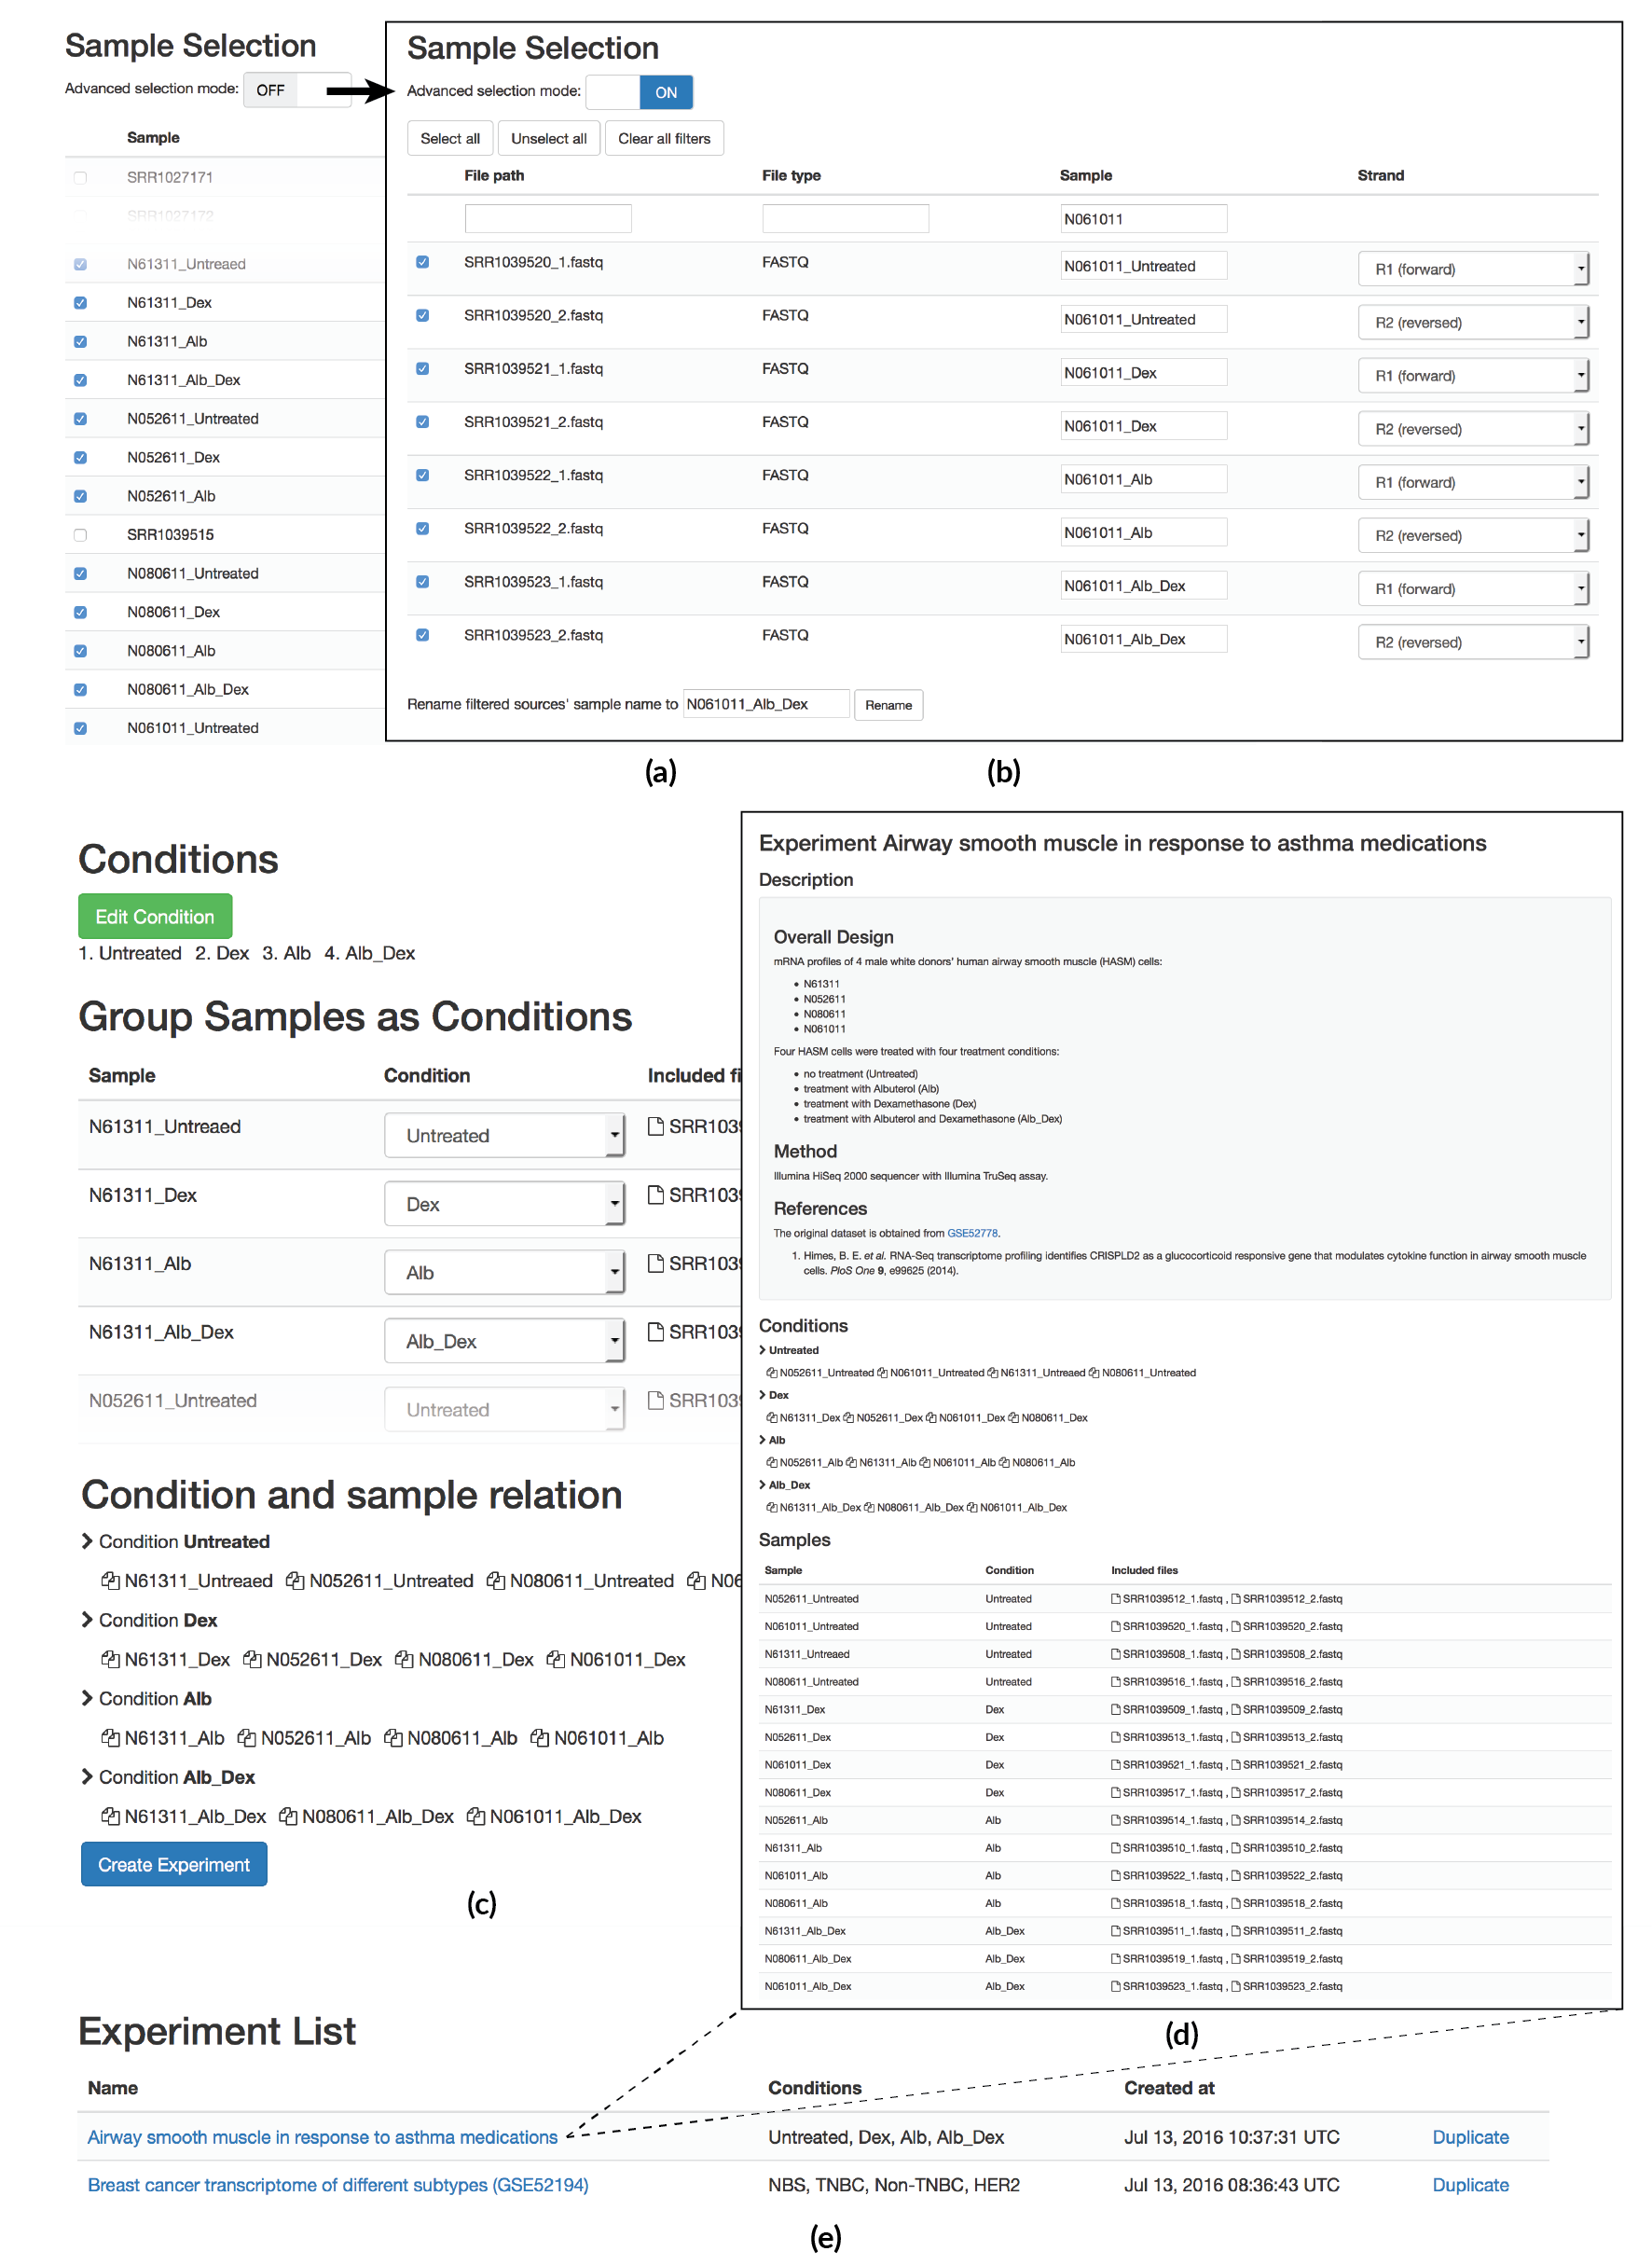
\includegraphics[width=1\textwidth]{images/biocloud_experiment_sample_condition}
\caption[Experiment design on BioCloud (cont'd)]{
    Experiment design on BioCloud (cont'd).
    (a)
    (b)
    (c)
    (d)
    (e)
}
\label{fig:biocloud-experiment-design}
\end{figure}




\section{Analysis submission}


\section{Job queue monitoring}

% email notification

\section{Report and result access}
\label{s:report-result-access}

\subsection{Integration with public genome browser}


\section{Admin}
\label{s:biocloud-admin}


\section{RNA-Seq analysis result}

\subsection{QC}

\subsection{Alignment - STAR}

\subsection{Alignment - HISAT2}

TODO: finish the dataset execution

\subsection{Cufflinks}

\subsection{featureCounts}

\subsection{DESeq2}

TODO: finish the dataset execution


\section{DNA-Seq analysis result}

\subsection{QC}

\subsection{Alignment - BWA MEM}

\subsection{Variant calling - Varscan}

\subsection{Variant calling - GATK}

TODO: finish the data execution

% There is a tree in Figure~%\ref{i:tree}.
% This is English line spacing test. You should see double spacing text.
% This is English line spacing test. You should see double spacing text.
% This is English line spacing test. You should see double spacing text.

%i:tree
%\begin{figure}[!htbp]
\centering
\tikzset{every tree node/.style={align=center},
    level distance=40pt,
    sibling distance=6pt}
\begin{tikzpicture}
\Tree[.root
       [ (a) ]
       [.node
         [.node
           [ (b) ]
           [ (c) ]
         ]
         [.node
           [ (d) ]
           [ (e) ]
           [ (f) ]
           [ (g) ]
           [ (h) ]
         ]
       ]
     ]

\end{tikzpicture}

\caption{A tree. }
\label{i:tree}
\end{figure}


% There is a barchart in Figure~%\ref{i:barchart}.
% This is English line spacing test. You should see double spacing text.
% This is English line spacing test. You should see double spacing text.
% This is English line spacing test. You should see double spacing text.

%i:barchart
%\begin{figure}[!htbp]
    \centering
    \vspace{2em}
    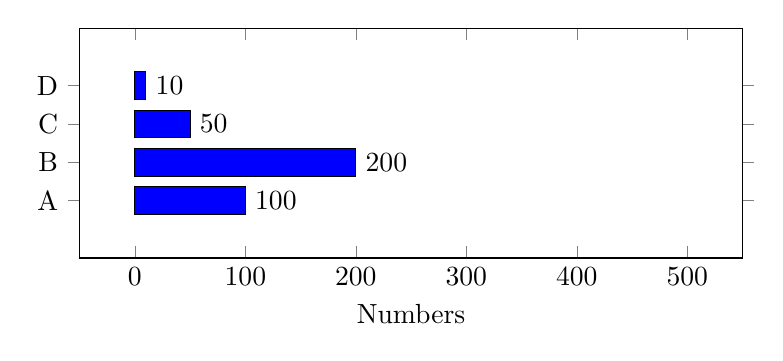
\begin{tikzpicture}
        \begin{axis}[
            enlarge y limits=0.5,
            enlarge x limits=0.1,
            height=4.5cm,
            width=10cm,
            symbolic y coords={A,B,C,D},
            xmin=0,
            xmax=500,
            xbar=1pt,
            xlabel=Numbers,
            nodes near coords={\pgfmathprintnumber[/pgf/number format/assume math mode]{\pgfplotspointmeta}},
            nodes near coords align={horizontal},
            every node near coord/.append style={
                anchor=west}
            ,
            xticklabel style={/pgf/number format/assume math mode},
            yticklabel style={/pgf/number format/assume math mode},
            ytick=data
          ]
            \addplot[xbar,fill=blue] coordinates {
            (100,A)
            (200,B)
            (50,C)
            (10,D)
            };
        \end{axis}
    \end{tikzpicture}
    \caption{A barchart.}
    \label{i:barchart}
\end{figure}


% Our method outperforms state-of-art systems as shown in Table~\ref{t:results}.
% This is English line spacing test. You should see double spacing text.
% This is English line spacing test. You should see double spacing text.
% This is English line spacing test. You should see double spacing text.

%t:results
% \begin{table}[!htbp]
\caption{Final performance of our system. }
\label{t:results} 
\centering
\begin{tabular}{|c|c|c|c|}
\hline

Method      &    Precision &     Recall &     F1-Score \\ \hline
their model &     3.40     &      3.40  &      3.40    \\ \hline
our model   &    99.99     &     99.99  &     99.99    \\ \hline


\end{tabular}
\end{table}

% \begin{table}[!htbp]
\caption[mirDeep2 result summary of both novel and known miRNA.]{mirDeep2 result summary of both novel and known miRNA. Here we can put some very lengthy descriptions as our table legend, and it will not ruin the list of tables, which will only display the shorten version of the caption.}
\label{t:all-sum}
\centering
\begin{threeparttable}
	\begin{tabular}{ccccccc}
	\toprule
    & \multicolumn{3}{c}{novel miRNAs} & \multicolumn{3}{c}{known miRNAs}\\
    \cmidrule(r){2-4} \cmidrule(r){5-7}
    miRDeep2 &       & estimated & estimated  &       &       &  \\
    score & predicted &  false positives\tnote{$\ast$} & true positives\tnote{$\dagger$} & in species & in data & detected\\
    \midrule
   >10    & 25    & 7 $\pm$ 3 & 18 $\pm$ 3 & 2025  & 1199  & 600 (50\%) \\
    9     & 28    & 8 $\pm$ 3 & 20 $\pm$ 3 & 2025  & 1199  & 609 (51\%) \\
    8     & 30    & 8 $\pm$ 3 & 22 $\pm$ 3 & 2025  & 1199  & 621 (52\%) \\
    7     & 31    & 8 $\pm$ 3 & 23 $\pm$ 3 & 2025  & 1199  & 635 (53\%) \\
    6     & 37    & 9 $\pm$ 3 & 28 $\pm$ 3 & 2025  & 1199  & 647 (54\%) \\
    5     & 50    & 11 $\pm$ 3 & 39 $\pm$ 3  & 2025  & 1199  & 720 (60\%) \\
    4     & 58    & 27 $\pm$ 6 & 31 $\pm$ 6 & 2025  & 1199  & 744 (62\%) \\
    3     & 64    & 74 $\pm$ 8 & 0 $\pm$ 1 & 2025  & 1199  & 752 (63\%) \\
    2     & 92    & 97 $\pm$ 9 & 2 $\pm$ 3 & 2025  & 1199  & 797 (66\%) \\
    1     & 181   & 132 $\pm$ 10 & 49 $\pm$ 10 & 2025  & 1199  & 891 (74\%) \\
    0     & 245   & 397 $\pm$ 20 & 0 $\pm$ 0 & 2025  & 1199  & 923 (77\%) \\
    -1    & 284   & 574 $\pm$ 22 & 0 $\pm$ 0 & 2025  & 1199  & 945 (79\%) \\
    -2    & 406   & 703 $\pm$ 23 & 0 $\pm$ 0 & 2025  & 1199  & 970 (81\%) \\
    -3    & 537   & 822 $\pm$ 25 & 0 $\pm$ 0 & 2025  & 1199  & 987 (82\%) \\
    -4    & 625   & 959 $\pm$ 28 & 0 $\pm$ 0 & 2025  & 1199  & 988 (82\%) \\
    -5    & 703   & 1088 $\pm$ 27 & 0 $\pm$ 0 & 2025  & 1199  & 991 (83\%) \\
    -6    & 774   & 1173 $\pm$ 26 & 0 $\pm$ 0 & 2025  & 1199  & 991 (83\%) \\
    -7    & 862   & 1227 $\pm$ 26 & 0 $\pm$ 0 & 2025  & 1199  & 992 (83\%) \\
    -8    & 923   & 1265 $\pm$ 27 & 0 $\pm$ 0 & 2025  & 1199  & 992 (83\%) \\
    -9    & 962   & 1291 $\pm$ 26 & 0 $\pm$ 0 & 2025  & 1199  & 992 (83\%) \\
    -10   & 1006  & 1311 $\pm$ 26 & 0 $\pm$ 0 & 2025  & 1199  & 992 (83\%) \\
		\bottomrule
	\end{tabular}
	\begin{tablenotes}
		\item[$\ast$] The number of false positives is estimated from 100 rounds of permuted controls.
		\item[$\dagger$] The number of true positives is estimated as $t = \mathit{total} - \mathit{false\:positives}$. The percentage of the predicted novel miRNAs that is estimated to be true positives is calculated as $p = t / \mathit{total}$. In each of the 100 rounds, $t$ and $p$ are calculated, generating mean and standard deviation of $t$ and $p$. The variable $p$ can be used as an estimation of miRDeep2 positive predictive value at the score cut-off. 
    \end{tablenotes}
\end{threeparttable}
\end{table}
% vim: set textwidth=79 spell:
